\subsubsection{Komplettsystem}
\begin{figure}[h!]
	\centering
	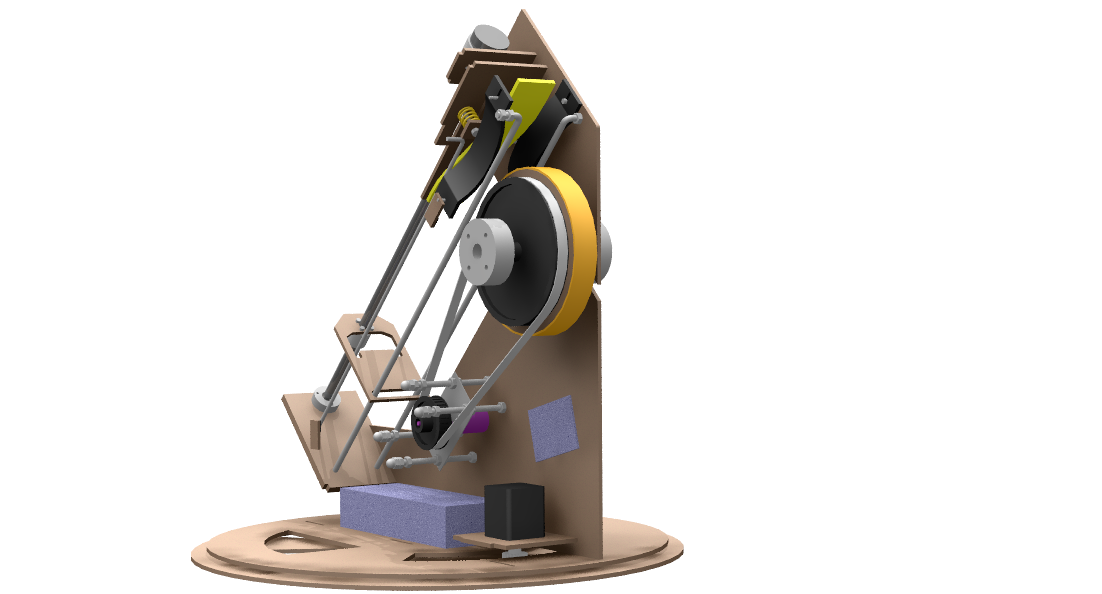
\includegraphics[width=\linewidth]{../../fig/Komplettsystem}
	\caption{Komplettsystem}
	\label{fig:Komplettsystem}
\end{figure}
\paragraph{Komponentenbeschrieb}

Um die verschiedenen gelaserten Komponenten zu verbinden werden vorallem Steckverbindungen eingesetzt. Den Einzelteilen wurden, um dies zu ermöglichen, Aussparungen und Nuten beigefügt. Für kleinere Komponenten wie Lager oder Halterungen werden hauptsächlich Schraub-, sowie vereinzelt Klebverbindungen verwendet. Die zwei Grundplatten wurden mittels eingepressten Alustiften verbunden. 

\paragraph{Entwicklungsprozess}

Für die Entwicklung der Wurfmaschine wurden anfangs diverse Handskizzen erstellt. Als man sich für ein mögliches Konzept entschieden hatte, wurden alle weiteren Ideen mittels dem CAD-Programm Siemens NX8 bzw. NX9 visualisiert und entwickelt. Durch dieses Vorgehen konnte Änderungen jeweils schnell angebracht werden. Bei den einzelnen Komponenten wurden bewusst nicht alle Befestigungsbohrungen im CAD-Modell erstellt, um nach dem Laserfertigen noch Spielraum für Veränderungen zu haben.